\section[Effects on downstream analysis]{Effects on downstream analysis - not quite the missing link, but close}
\label{variantcalling-sec:downstream}

The ability to find additional shared variants has significant impact on our understanding of cancer evolution and the timing of initiation and metastatic seeding. Recent work has shown, that similar to the well known genetic heterogeneity, there is heterogeneity when it comes to metastatic seeding. While traditionally it was thought that tumours only metastesised after they reached a certain size, to escape the restrictions of the niche, like reduced nutrition, recent publications showed, there is also very early metastatic seeding \cite{Hu2019}. 
But all those methods are ultimately based on the somatic variants found in the data, so if we improve on the input of the downstream analysis methods, we can expect a clearer and possibly more granular result.

In this section I will highlight for a few examples on how big the effect can be for methods, like phylogenetic reconstruction and clonal decomposition, which use somatic variants as input.


\subsection[Phylogenetic reconstruction]{Phylogenetic reconstruction}
\label{variantcalling-sec:phylo}
As this work is not about the advantages and shortcomings of different phylogenetic reconstruction tools, we will not show a comprehensive amount of these tools, but rather focus on the results.  For this reason, we chose to use neighbour joining (NJ) \cite{Saitou1987}, because it is fast, readily available in most phylogenetic reconstruction tool kits and if the input distance is correct, the output will be correct. And even, if the distance is not 100\% correct, if the distance is ``nearly additive`` and the input distances are not far off the real distance, the tree topology will still be reconstructed correctly \cite{Mihaescu2007}. Lastly, in contrast to many other methods like UPGMA and WPGMA \cite{Sokal1958}, NJ does not assume an equal mutation rate of each sample, because we know, that the molecular clock hypothesis \cite{Zuckerkandl1962} is not valid for different lineages of cancers \cite{Shibata2010}.

While there are lots of distance measures for DNA sequences, which allow accounting for different probabilities of transitions and transversions as well as uneven base composition, models like F81 \cite{Felsenstein1981} or HKY85 \cite{Hasegawa1985} are only really designed for germline mutations and are not easily applicable for subclonal somatic mutations, which is why we decided to first transform the variants present in all samples into a binary occurrence vector and then calculating the Hamming distance \cite{Hamming1950} between all samples. This generates a maximum parsimony approach and the branch length of the trees will be directly translatable to the amount of variants which are different between samples. 

\autoref{fig:ca9phylo} shows both the reconstructed phylogenies of the autopsy samples of patient ``CA-F`` from the manuscript (\autoref{ch:appendixManuscript}), using the variants found with the default tumour-normal method on the left and our improved joint method on the right. The exact same reconstruction methodology was used otherwise, such that only the input lead to the final difference.

\begin{figure}[!ht]
\centering
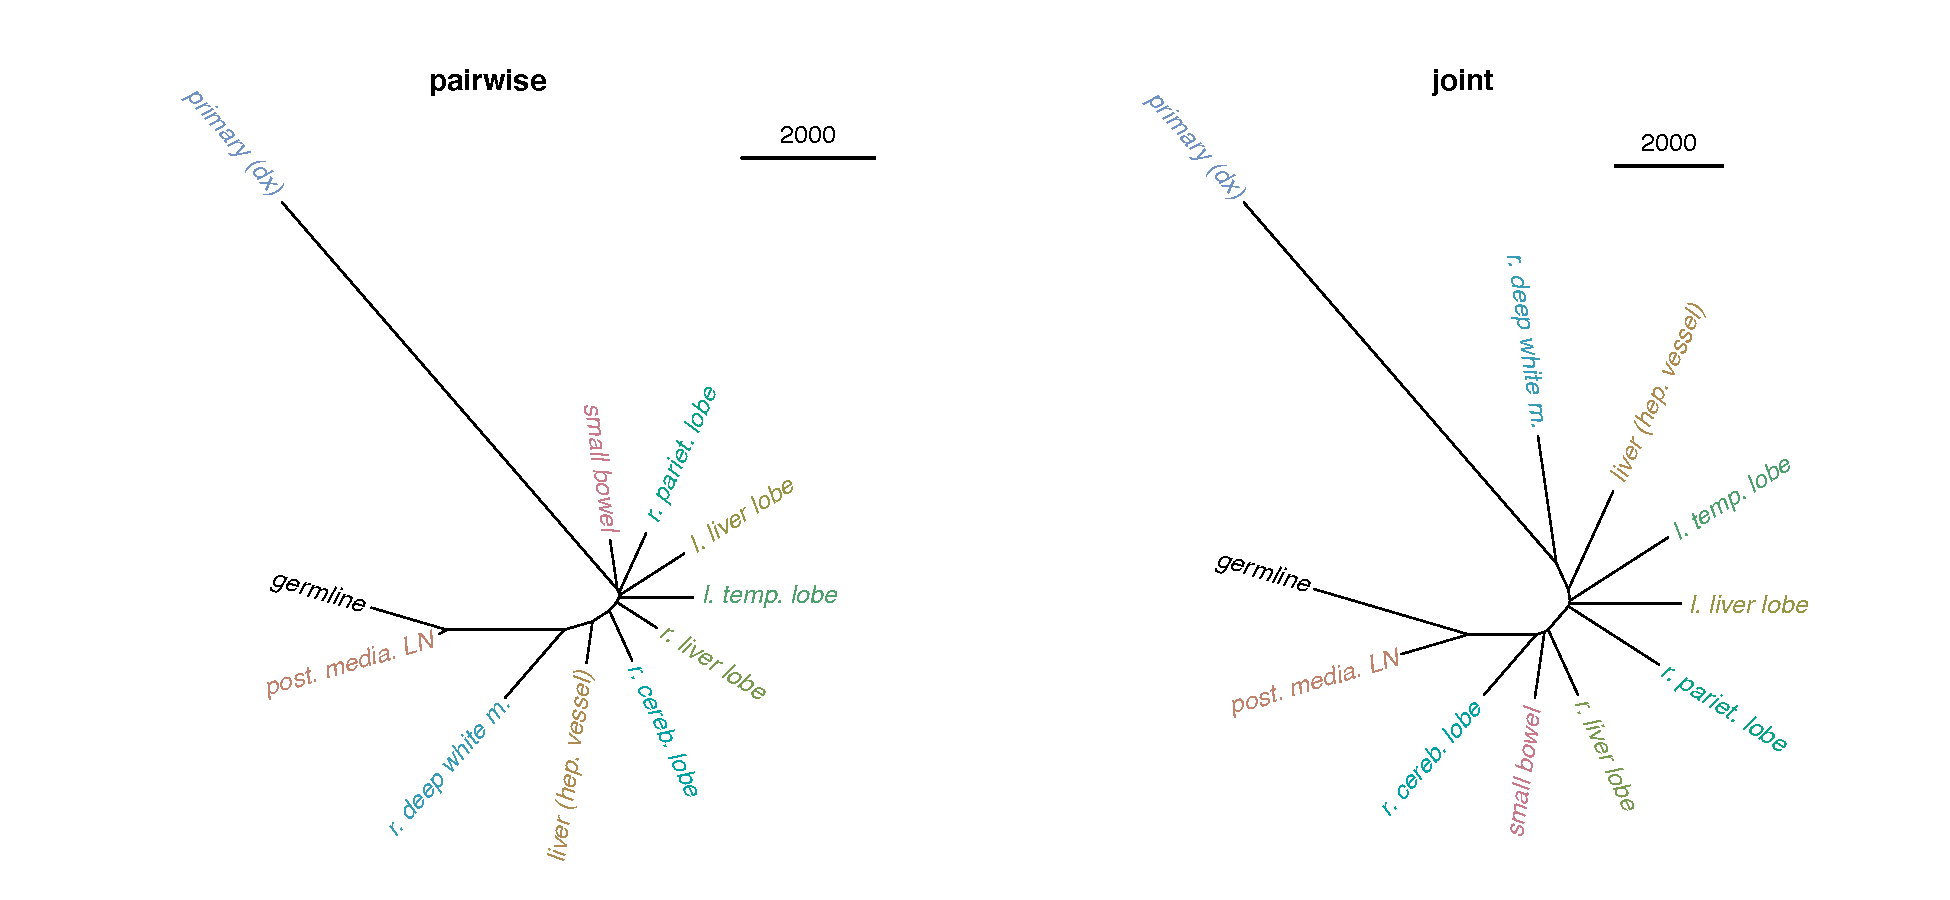
\includegraphics[width=.99\linewidth]{Figures/phyloCA9.pdf}
\caption[Reconstructed phylogenies of joint samples]{Reconstructed phylogenies of a patient with multiple spatially distinct samples; Reconstruction method is neighbour joining for both cases, only the input of the called variants is different. Tip labels describe the location of the sample in the patient. Trees are shown as unrooted with germline as fixated origin point; black line ruler shows the length of an edge with 5000 mutations}\label{fig:ca9phylo}
\end{figure}

\todo[inline, color=green]{Maybe adjust the font size in the tress to make it more readable}

There are several obvious changes, first, the longer edge connecting the the germline, which we consider as the state of no somatic variants, to all other samples. This shows that there are many more shared mutations in all samples, than what would have been anticipated with the default method. As the accumulation of somatic variants is still used as a proxy for timing and cell divisions, when assuming a high mutation rate for lung cancer ($5.3 \cdot 10^{-8}$ from \citeauthor*{Werner2020} \cite{Werner2020}) this difference of $\approx 36000$ variants is equivalent to $\approx 2000$ cell divisions. While the cell doubling rate of lung cancers is highly dependent on the type \cite{Arai1994}, this difference makes a huge difference when assessing the timing of the tumour initiation and further evolution. 

Secondly, there have been topological changes, which generate a bifuricating edge between the olive coloured ``r. liver lobe`` and the ``r. pariet. lobe``showing a bottle neck in cancer evolution, which fits very well with the clinical history, where the patient lived with stable disease for almost ten years, before progressing and dying. The extreme distance of the primary/diagnostic sample from the rest of the samples could be either a difference in sequencing quality, or due to the exposure to FFPE for the ten years between tumour diagnosis and death. However, as this feature is preserved between both the joint and the pairwise analysis it is no factor for our new method.

\autoref{fig:tanglePhyloCA9} shows a topology focused view of the two trees, which highlights the breaks which are needed to morph one tree into the other with dotted edges \cite{Vienne2018}. The common subtrees are coloured the same on both sides and connecting lines show identical labels. This format shows that while the trees look quite similar at first glance, they show vastly different topologies.

\begin{figure}[!ht]
\centering
\includegraphics[width=.99\linewidth]{Figures/tanglePhyloCA9.pdf}
\caption[Tanglegram of the reconstructed phylogenies]{Side by side view of the reconstructed trees from \autoref{fig:ca9phylo}; internal edges, which are distinct between trees are shown as dotted lines; common subtree is shown in red  Tree labels have been sorted to minimise distance between labels; Visualisation generated with dendextend \cite{Galili2015}}\label{fig:tanglePhyloCA9}
\end{figure}
\todo[inline, color=green]{maybe increase the line width of the edges}

One example of this is ``small bowel`` which was connected to the red common subtree, but is now much closer to the ``r. cereb lobe`` and forms a parallel clade with the ``r.liver lobe``. In general, where the pairwise tree shows a very linear topology, which leaves only branching out of the main with no disjunct subclades, which are clearly present in the joint reconstruction.  (\autoref{fig:tanglePhyloCA9}).


\section[Longitudinal analysis]{Longitudinal analysis - something for the ages }
\label{variantcalling-sec:longitudinal}

While the initial motivation for the development of these workflows was the analysis of multi-region, so spatial, samples from the same patient coming from the CASCADE rapid autopsy program, a longitudinal application of these methods for the joint analysis of diagnostic and relapse sample, or even the repeated testing of ctDNA are quite worth thinking about. In this part, I will present work using the published workflows on a longitudinal datasets, which highlights the flexibility and wide spread use of our new methods.

Patient ``CA-F`` had additionally to their autopsy also three longitudinal blood samples taken, from which ctDNA was extracted and WES performed. In a study of late stage melanoma patients, \Citeauthor{Tan2019} identified ctDNA sequencing as a way to stratify patients into high and low risk of relapse and therefore inform adjuvant therapy \cite{Tan2019}. Similar to the spatially related samples, the joint analysis can improve the performance of the somatic variant calling, which then in term enables the detection of lower allele frequency variants, either through lower tumour burden or through the limited availability of DNA fragments from brain lesions due to the blood brain barrier\cite{2014}.

To show that even in longitudinal data, the joint analysis can boost the signal, we jointly variant called the diagnostic biopsy with the three ctDNA samples and compared them with the results from the pairwise analysis. On average we found 2905 additional variants in each of the ctDNA samples which is more than double than the number of variants found with the pairwise analysis (2414). Out of those, we found 534 variants in the ctDNA samples, which were found as a high confidence variant in the diagnostic sample, indicating that these findings are high quality calls. 

\begin{figure}[!ht]
\centering
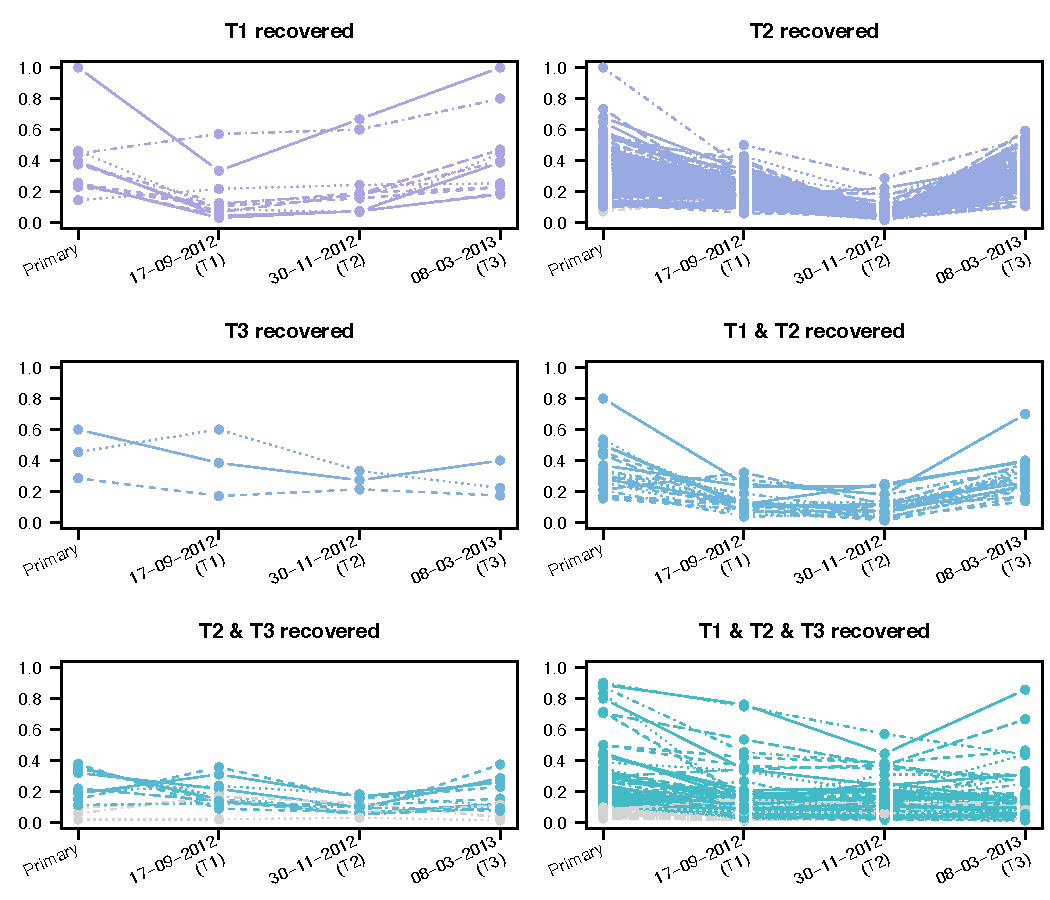
\includegraphics[width=.99\linewidth]{Figures/longitudinalCA9ctDNAVafs.pdf}
\caption[Improved somatic variant calling in longitudinal data]{Improved somatic variant calling in longitudinal data: Variant allele frequency (VAF) of variants found additionally through joint variant calling which were found as high confidence variants in the primary sample; Variants with less than 0.1 VAF in the primary are coloured grey; ``T1 recovered`` shows variants, which were high confidence in all ctDNA samples but T1 and were only found through joint calling there; Axis label show the date of blood collection }\label{fig:longitudinalVAFsctDNA}
\end{figure}


Exactly how we found in the publication, that lower tumour purity samples benefit more from the joint analysis, we see that time point 2 (T2) have the highest amount of recovered variants (377) which are found as high confidence variants in both other time points (\autoref{fig:longitudinalVAFsctDNA} T1 recovered vs. T2 recovered vs. T3 recovered) as T2 also has the lowest tumour burden recorded (T1: 60\%; T2: 20\%; T3: 60\%) however, there are still 106 variants, which were not found in the ctDNA samples at all with the pairwise analysis at all, even though they were high confidence variants in the primary sample (\autoref{fig:longitudinalVAFsctDNA} T1 \& T2 \& T3 recovered). These cases usually show a lower depth of coverage (dp) in the ctDNA samples, which might indicate a problematic region in the genome, but rather than it not being a variant, it is just a sign of incomplete data, which can be used with our joint approach. 

\begin{figure}[!ht]
\centering
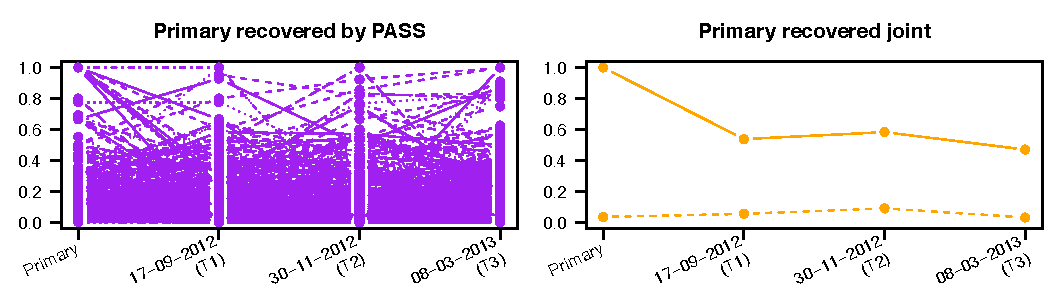
\includegraphics[width=.99\linewidth]{Figures/longitudinalCA9primaryVafs.pdf}
\caption[Longitudinal data informs diagnostic variant calling]{Longitudinal data informs diagnostic variant calling: Vafs of variants additionally found through joint calling in the primary samples; Primary recovered by PASS shows variants which were high confidence in at least one ctDNA sample; Primary recovered joint shows variant which were low confidence in all samples in the pairwise analysis; Axis label show the date of blood collection}\label{fig:longitudinalVAFsprimary}
\end{figure}


Finally, we can also find 398 additional variants in the   primary sample. 398 were discarded due to missing data in the the tissue sequencing, but could be found with a high confidence in the longitudinal data and two of the variants were included, as all 4 samples had this variant below the detection threshold (\autoref{fig:longitudinalVAFsprimary}). The missing depth in the primary also leads to the occasional very high allele frequency of the variant, as all available reads show the variant, but they are below the threshold normal variant callers will report variants.

This shows that both spatially and longitudinal related samples should be analysed jointly, as it substantially increases the amount of true variants found, which as shown before have a big impact on downstream analysis of the samples.



\subsection[Clonal deconvolution]{Clonal deconvolution}
\label{variantcalling-sec:clonal}

Finally, the holy grail of analysis of multiple related samples from the same patient is the clonal deconvolution, where subclonal reoccurring patterns of mutations are detected. These can be linked to either parallel evolution through positive selection pressure, like a targeted drug or to the process of developing Metastases where a piece of the cancer ``breaks`` off and grows at a different site.
Surprisingly, as it shares the same issues as the joint somatic variant calling of needing deeply sequenced data from multiple samples of the same organism, there is a plethora of algorithms and methods available for clonal deconvolution. To name a few, since 2015 PhyloWGS \cite{Deshwar2015}, Canopy \cite{Jiang2016}, CLOE \cite{Marass2016}, CloneFinder \cite{Miura2018}, MACHINA \cite{ElKebir2018} and MOBSTER \cite{Caravagna2020} were published. Underlying these models is a form of clustering variants with similar variant allele frequency together, to reduce the combinatorial space and enhance the confidence in the signal \cite{Tarabichi2021}. However even though there is a high number of tools, the challenge to select the right tool is substantial, especially since all of them have up and downsides \cite{Miura2020}. In this work we decided to use PhylogicNDT \cite{Leshchiner2018} as it has been shown to work well on clinical samples \cite{Gerstung2020} and does not have the restriction for the input to be from copy number neutral areas which many of the other tools have.

The analysis was conducted by transforming the variants called with the joint workflows as well as the default pairwise analysis into the required MAF file format without the cancer cell fraction part, in order to let PhylogicNDT calculate those on the fly. The local copy numbers for each variants are generated by intersecting the called segments from sequenza with the position of the variants. Variants which could not be assigned a local copy number change were discarded from the analysis.

\begin{figure}[!ht]
\centering
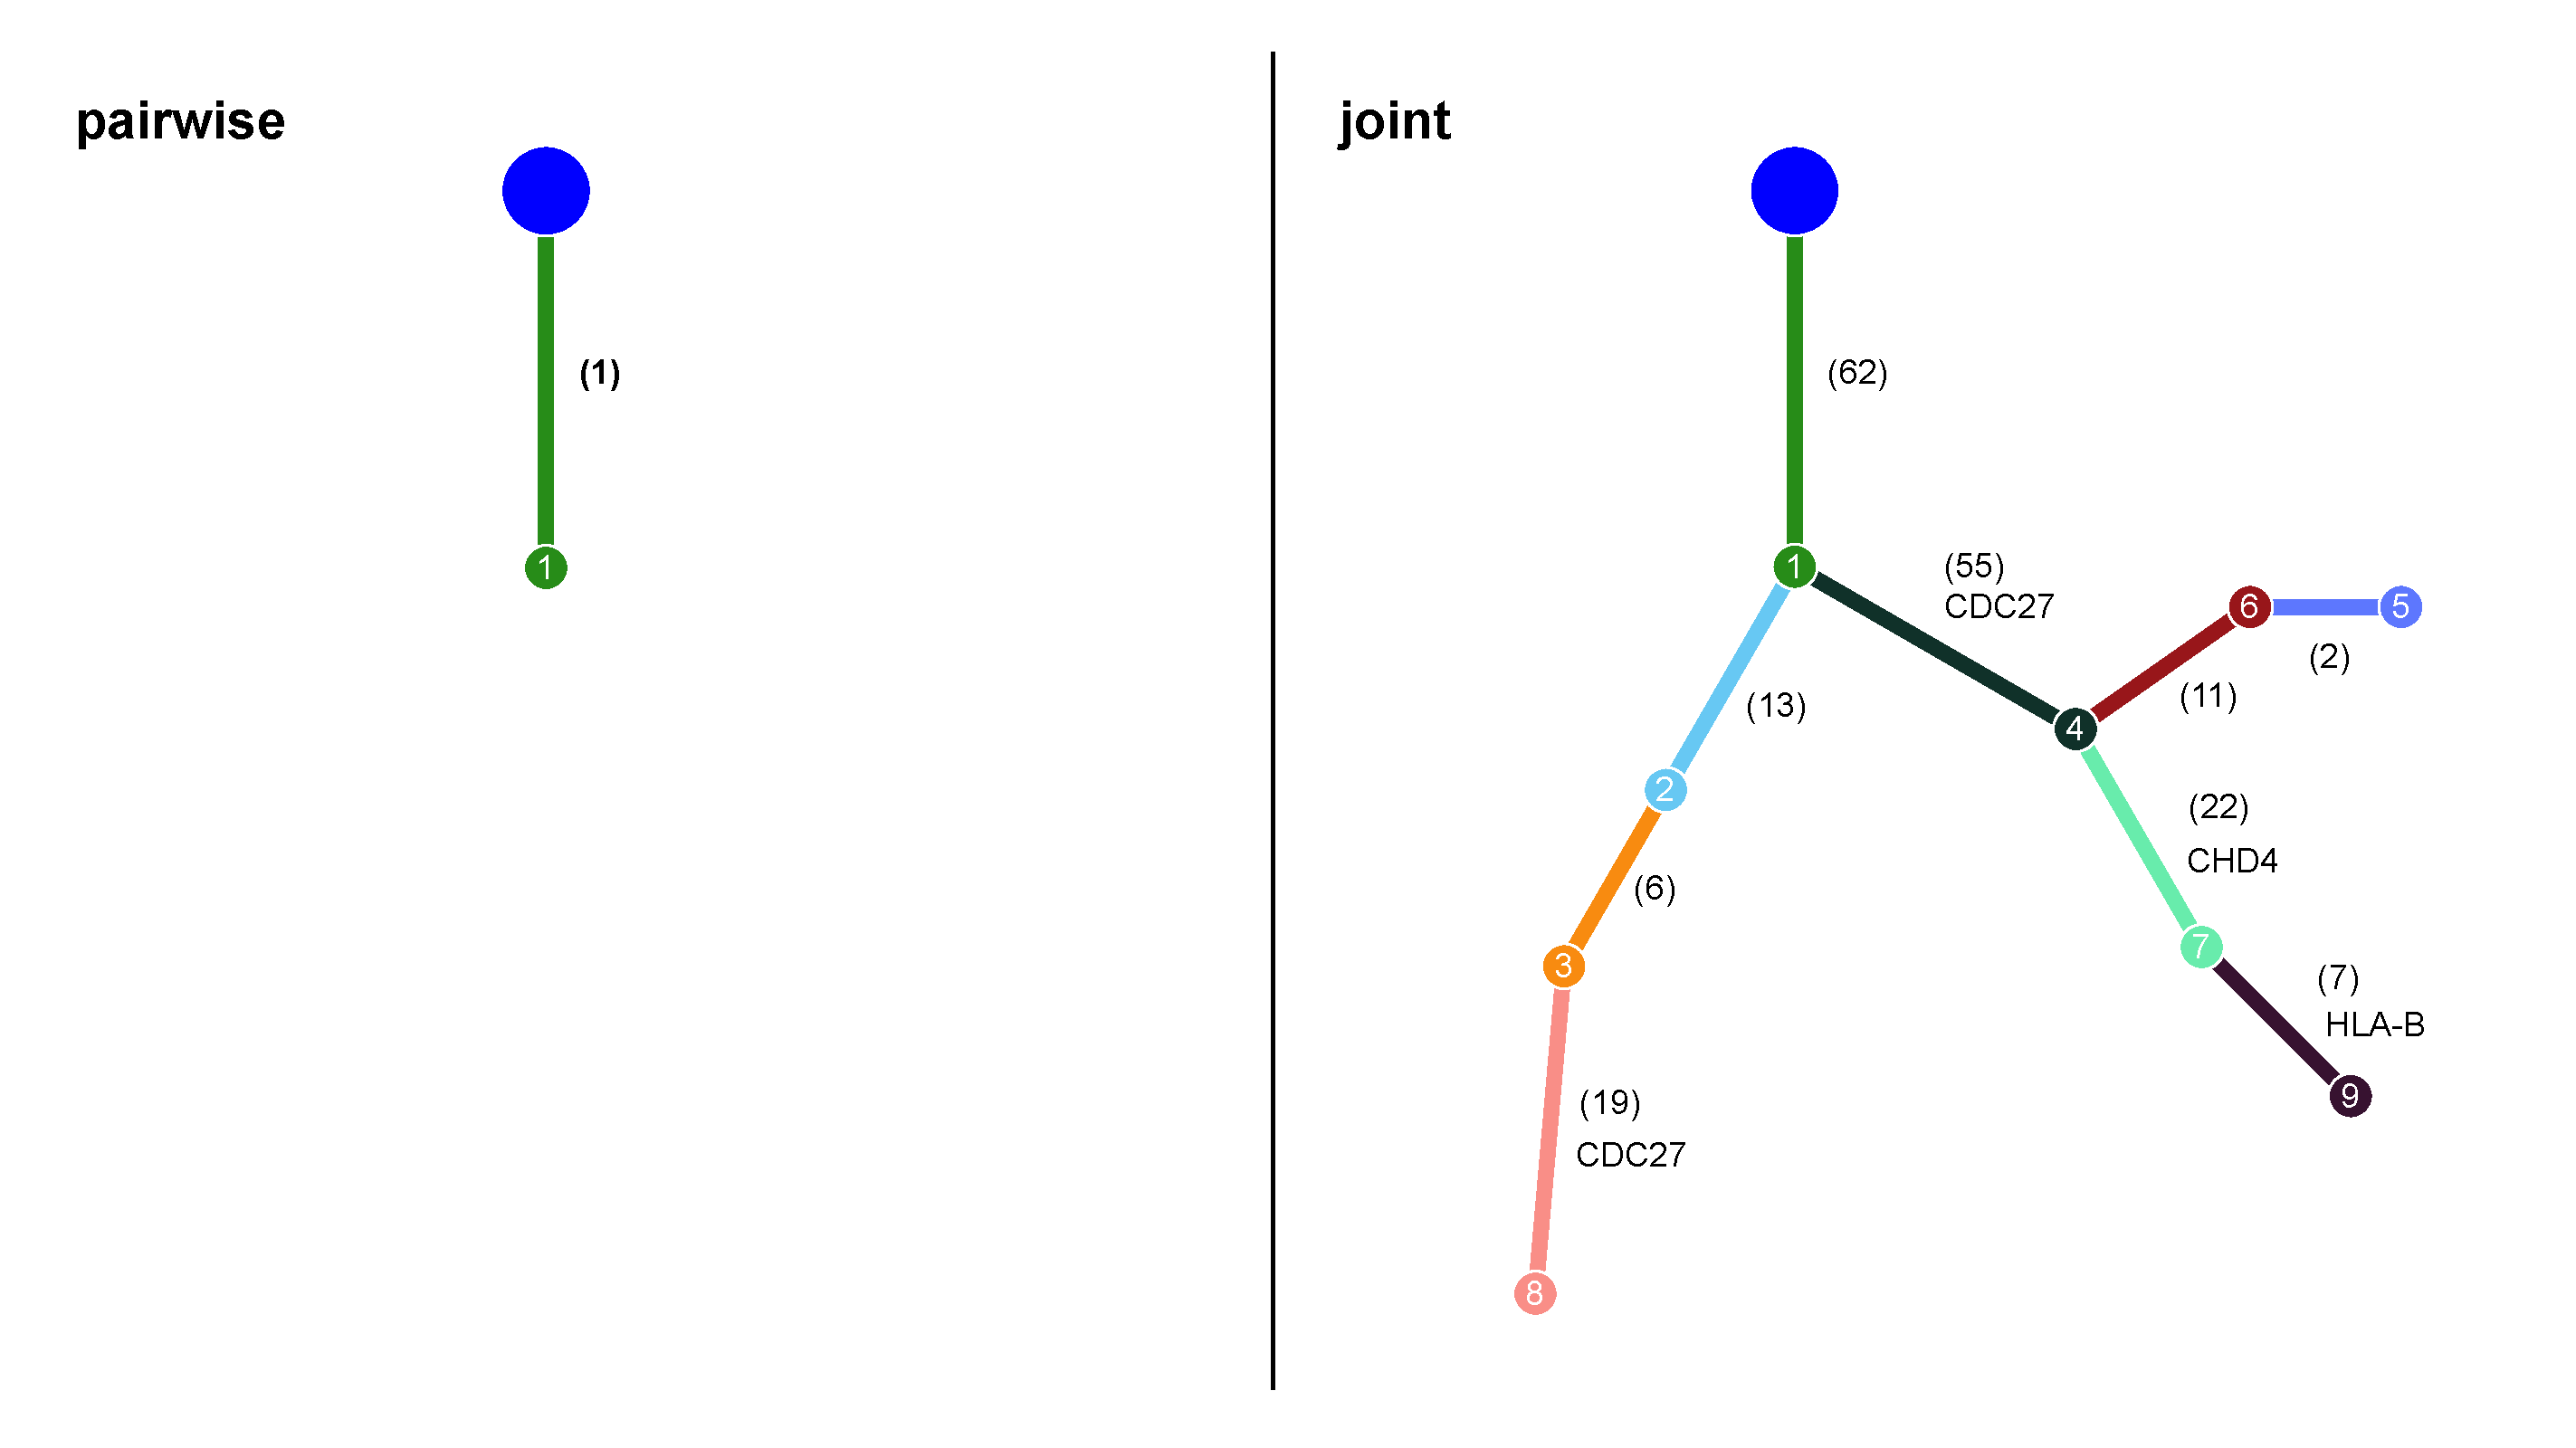
\includegraphics[width=.99\linewidth]{Figures/clonalDeconv.pdf}
\caption[Reconstructed clonal trees for joint and pairwise variant calling]{Reconstructed clonal trees from PhylogicNDT; Blue circle at top depicts the germline/normal state. The coloured edges with the same coloured circle represents a distinct subclone of the parent from which the edge emerges; The number in braces next to the edge is the number of mutations which define this subclone with an added gene symbol added, if there is a cancer driver gene mutation. The left part shows the result when using the default pairwise method of Strelka2 and the right side uses the results from the Strelka2Pass workflow}\label{fig:clonaldeconv}
\end{figure}


\autoref{fig:clonaldeconv} shows the highest parsimony clonal tree reconstructed by PhylogicNDT for the pairwise as well as the joint variant calling. As the copynumber calling information is the same for both inputs, the only difference is in the called variants. While there was no subclonal structure detected at all for the pairwise analysis, there is a highly variable structure detected using the jointly called variants.
